\chapter{Theoretical Background}\label{chap:theory}
\begin{chapabstract}

    In this chapter, I describe physical mechanisms of radio emissions related to our study.
    At low frequencies, we observe free-free\footnote{\url{https://www.cv.nrao.edu/~sransom/web/Ch4.html}} (Bremsstrahlung) and synchrotron\footnote{\url{https://www.cv.nrao.edu/~sransom/web/Ch5.html}} radiations.
    Both radiations are the continuum emission.
    While the free-free radiation is usually dominant from a galaxy at $30 \sim 200\GHz$, the synchrotron radiation is dominant less than $30\GHz$ (Figure~\ref{fig:Condon1992_figure1}).\\ \vspace{0.2cm}
\begin{figure}[htbp]
	\centering
	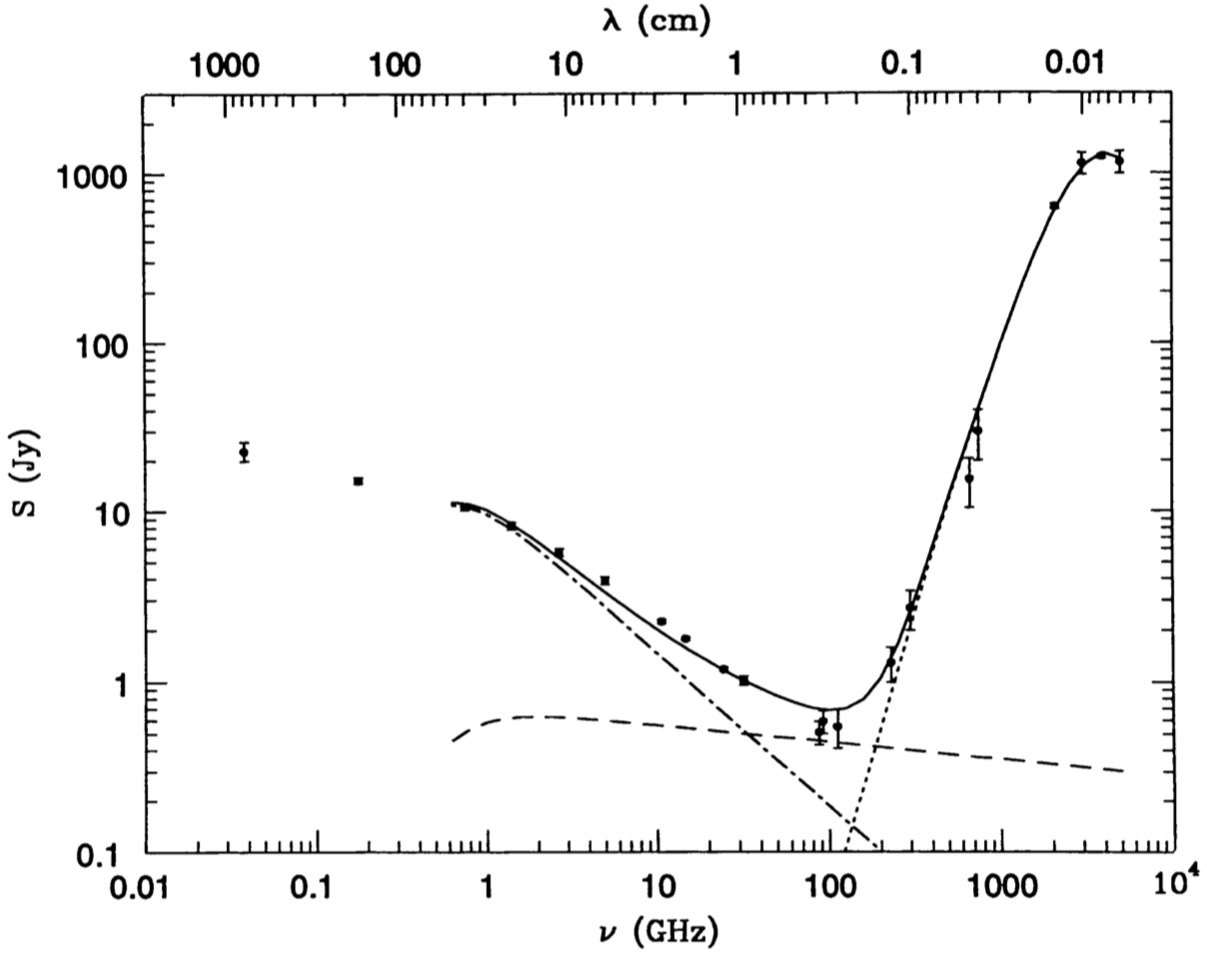
\includegraphics[width=.7\linewidth]{Chapter_2/Figures/Condon1992_Figure1.png}
    \caption[Reprint from \citet{Condon1992a} (Figure~1)]{\label{fig:Condon1992_figure1}
        (Reprint from \citet{Condon1992a}, Figure~1)\\
        This figure shows the spectral energy distribution of M82.
        The dotted line shows the dust thermal emission which is dominant at higher than $200\GHz$.
        The dashed line shows the free-free radiation from the \ih~regions around massive stars, which is dominant at $30 \sim 200\GHz$.
        The dot-dash line shows the synchrotron radiation emitted by the high energy electrons, which is dominant at less than $30\GHz$.
    }
\end{figure}

\end{chapabstract}



\section{Free-free radiation}\label{sec:freefreeradiation}

The free electrons produce free-free radiation by scattering off ions.
In star-forming galaxies, the radiation source is the \ih~region where young massive (OB) stars ionized most of the hydrogen atoms.
In this section, we consider the radiation mechanism of free-free radiation.
Here, I consider only electrons emit the radiation because an electron is much more accelerated than an ion due to the difference of their mass (an electron is 1840 times lighter than a proton).

Firstly, I consider the simplest case that a single electron passes by the ion and emits the radiation.
Note that the path of the electron does not change after the interaction because the energy of radio emission is much smaller than the mean electron energy in a plasma:

\begin{equation}\label{eq:essential_radio4n12}
    \frac{E\msb{10\GHz}}{\bra{E_e}} = \frac{h \times 10^{10}\,\mr{Hz}}{3kT / 2} = \frac{6.63 \times 10^{-27} \mr{erg\,s} \times 10^{10}\,\mr{Hz}}{1.5 \cdot 1.38 \times 10^{-16}\,\mr{erg\,K^{-1}} \cdot 10^4\,\mr{K}} = 3.3 \times 10^{-5}
\end{equation}

During the interaction, the electron is accelerated by the electric field by the ion.
Then, we can write the equation of motion for parallel and perpendicular to the electron's path (Figure~\ref{fig:nrao_radio4n2}):

\begin{figure}[htbp]
	\centering
	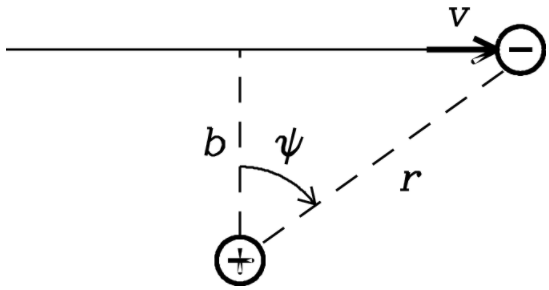
\includegraphics[width=.5\linewidth]{Chapter_2/Figures/NRAO_radio4n2.png}
    \caption[The schematic image of the interaction of an electron with the ion]{\label{fig:nrao_radio4n2}
        This figure shows the schematic picture of the interaction of an electron with the ion.
        $b$ and $\tau = b/v$ are called the impact parameter and the collision time, respectively.
    }
\end{figure}
\begin{align}
    F_{\|} &= m_{\mr{e}} \dot{v}_{\|}=\frac{-Z e^{2}}{r^{2}} \sin \psi=\frac{-Z e^{2} \sin \psi \cos ^{2} \psi}{b^{2}}\label{eq:essential_radio4n15}\\
    F_{\perp} &= m_{\mr{e}} \dot{v}_{\perp}=\frac{Z e^{2}}{r^{2}} \cos \psi=\frac{Z e^{2} \cos ^{3} \psi}{b^{2}}\label{eq:essential_radio4n16}
\end{align}
where $b$ is the impact parameter and $\cos\psi = \frac{b}{r}$.

These accelerations show different shapes of the pulse (Figure~\ref{fig:nrao_radio4n3}).
Since the parallel acceleration produces some infrared radiation with the angular frequency $\omega \sim \tau^{-1} = \frac{v}{b}$ ($\tau$ is the collision time), its contribution is negligible at radio frequency.

\begin{figure}[htbp]
\centering
	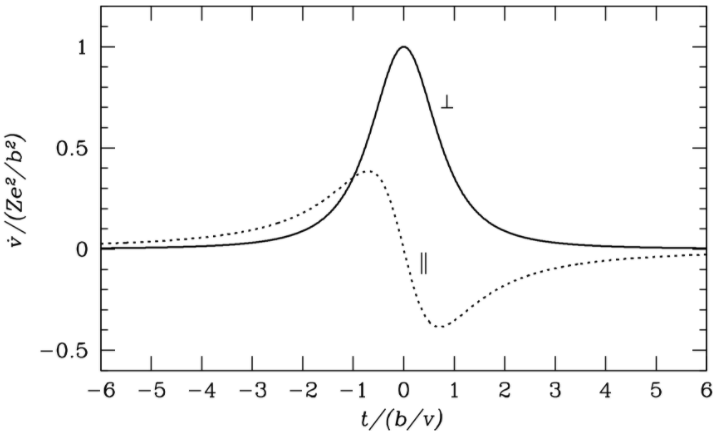
\includegraphics[width=.7\linewidth]{Chapter_2/Figures/NRAO_radio4n3.png}
    \caption[The acceleration of an electron by an ion]{\label{fig:nrao_radio4n3}
        This figure shows the acceleration of an electron.
        The solid and dotted lines show the case of perpendicular and parallel to the electron's velocity, respectively.
    }
\end{figure}

Therefore, the power of free-free radiation from the acceleration perpendicular to the electron's velocity is:

\begin{equation}\label{eq:essential_radio4n17}
    P=\frac{2}{3} \frac{e^{2} \dot{v}_{\perp}^{2}}{c^{3}}=\frac{2 e^{2}}{3 c^{3}} \frac{Z^{2} e^{4}}{m_{\mr{e}}^{2}}\brp{\frac{\cos ^{3} \psi}{b^{2}}}^{2}
\end{equation}
where we insert $\dot{v}_{\perp}$ into the Larmor's formula $\brp{P = \frac{2}{3}\frac{q^2\dot{v}^2}{c^3},\,q\,\mr{is\,a\,charge}}$, which shows the power emitted by the accelerated particles.

We can get the total energy of $W$ by the pulse as follows:

\begin{equation}\label{eq:essential_radio4n18}
    W = \int^{\infty}_{-\infty} P\,\mr{d}t
\end{equation}

As I have noted above, the electron's velocity does not change so that we can change of variables:

\begin{equation}\label{eq:essential_radio4n19}
    v = \frac{\rd x}{\rd t}\ \ \ \mr{and}\ \ \ \tan\psi = \frac{x}{b}
\end{equation}

then,

\begin{equation}\label{eq:essential_radio4n20}
    v=\frac{b\,\rd\brp{\tan \psi}}{\rd t} = \frac{b\,\rd \psi}{\cos ^{2}\psi\,\rd t}
\end{equation}

and

\begin{equation}\label{eq:essential_radio4n21}
    \rd t=\frac{b}{v} \frac{\rd \psi}{\cos ^{2} \psi}
\end{equation}

Substituting Equation~\ref{eq:essential_radio4n17} and~\ref{eq:essential_radio4n21} into Equation~\ref{eq:essential_radio4n18} yields

\begin{equation}\label{eq:essential_radio4n22}
    W=\frac{2}{3} \frac{Z^{2} e^{6}}{c^{3} m_{\mathrm{e}}^{2} b^{4}} \int_{-\pi / 2}^{\pi / 2} \frac{b}{v} \frac{\cos ^{6} \psi}{\cos ^{2} \psi} \rd \psi=\frac{4}{3} \frac{Z^{2} e^{6}}{c^{3} m_{\mathrm{e}}^{2} b^{3} v} \int_{0}^{\pi / 2} \cos ^{4} \psi\ \rd \psi = \frac{\pi Z^2 e^6}{4 c^3 m_{\mr{e}}^2}\brp{\frac{1}{b^3v}}
\end{equation}
where $\int_{0}^{\pi / 2} \cos ^{4} \psi\,\rd \psi=\frac{3 \pi}{16}$.

The pulse energy $W$ shows the total energy emitted by a single electron interaction characterized by the impact parameter $b$ and the electron's velocity $v$.\\ \vspace{0.2cm}

Secondly, I consider the strength and spectral of free-free radiation from \ih~region with several simple assumptions.
Here, I assume the local thermodynamic equilibrium (LTE) in the \ih~region.
In LTE, electrons have a much higher speed than ions because of the difference of their mass, although the average kinetic energy of electrons and ions are equal.
Therefore, it is reasonable to think ions do not move by the interactions.

When I consider the cylindrical shell around the ion (Figure~\ref{fig:nrao_radio4n5}), I can calculate the number of electrons passing the ion per unit time between $b$ and $b + \rd b$ under the velocity range of $\rd v$:

\begin{figure}[htbp]
	\centering
	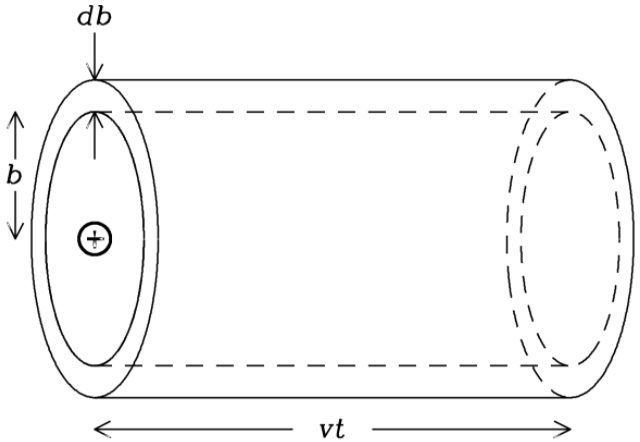
\includegraphics[width=.6\linewidth]{Chapter_2/Figures/NRAO_radio4n5.png}
    \caption[The schematic picuture of the cylindrical shell of electrons]{\label{fig:nrao_radio4n5}
        This figure shows the schematic picture that an electron passes the ion in the cylindrical shell.
    }
\end{figure}

\begin{equation}\label{eq:essential_radio4n27}
    n\msb{e} \brp{2\pi b,\rd b}\,v f\brp{v}\,\rd v
\end{equation}
where $f\brp{v}$ is the normalized speed distribution of electrons (In LTE, $f\brp{v}$ is the Maxwellian distribution).

The number $\dot{n}\msb{c}\brp{v,\,b}$ of such collisions per unit volume per unit time is:

\begin{equation}\label{eq:essential_radio4n28}
    \dot{n}\msb{c}\brp{v,\,b} = \brp{2\pi b} v f\brp{v} n\msb{e} n\msb{i}
\end{equation}

Then, I can write the emission coefficient $j_{\nu}$ as follows:

\begin{equation}\label{eq:essential_radio4n29}
    4 \pi j_{\nu}=\int_{b=0}^{\infty} \int_{v=0}^{\infty} W_{\nu}\brp{v,\,b} \dot{n}\msb{c}\brp{v,\,b} \rd v \rd b
\end{equation}
where $W\msb{\nu}\brp{v,\,b}$ is the average energy per unit frequency emitted during a single interaction and approximately written in $W\msb{\nu}\brp{v,\,b} = \frac{W}{\nu\msb{\max} \brp{= v/2\pi b}}$.

Substituting $W\msb{\nu}\brp{v,\,b}$ and Equation~\ref{eq:essential_radio4n28} into Equation~\ref{eq:essential_radio4n29} yields

\begin{align}
    4 \pi j_{\nu} &= \int_{b=0}^{\infty} \int_{v=0}^{\infty} \brp{\frac{\pi^2 Z^2 e^6}{2 c^3 m\msb{e}^2 b^2 v^2}} 2 \pi b\,\rd b\,n\msb{e} n\msb{i}\,v\,f(v) \rd v \label{eq:essential_radio4n30}\\
                  &=\frac{\pi^{3} Z^{2} e^{6} n\msb{e} n\msb{i}}{c^{3} m\msb{e}^{2}} \brp{\frac{2m\msb{e}}{\pi k T}}^{1/2}\int_{b=0}^{\infty} \frac{\rd b}{b}\label{eq:essential_radio4n31}
\end{align}
where I use the Maxwellian distribution:

\begin{equation}\label{eq:essential_radio4n34}
    f(v)=\frac{4 v^2}{\sqrt{\pi}} \brp{\frac{m\msb{e}}{2 k T}}^{3/2} \exp \brp{-\frac{m\msb{e} v^2}{2 k T}}
\end{equation}

Note that $\int^{\infty}_{b=0} \frac{\rd b}{b}$ diverges, so it needs finite limites $b_{\min}$ and $b_{\max}$.
To estimate $v_{\min}$, let's consider the change in momentum during the single electron-ion interaction:

\begin{align}\label{eq:essential_radio4n40}
    m\msb{e} \Delta v &= \int_{-\infty}^{\infty} F \rd t = \int_{-\infty}^{\infty}\left(\frac{Z e^{2} \cos \psi}{r^{2}}\right) \rd t=Z e^{2} \int_{-\infty}^{\infty} \frac{\cos ^{3} \psi}{b^{2}} \rd t \\
                      &= \frac{Z e^{2}}{b v} \int_{-\pi / 2}^{\pi / 2} \cos \psi\,\rd \psi=\frac{2 Z e^{2}}{b v} \\
                      &= \frac{2Ze^2}{bv} \brp{< 2m\msb{e}v}
\end{align}
where the maximum momentum transfer $m\msb{e} \Delta v$ is twice the initial momentum $m\msb{v}$. \\

Therefore, the minimum impact parameter $b_{\min}$ is

\begin{equation}\label{eq:essential_radio4n43}
    b_{\min} = \frac{Ze^2}{m\msb{e}v^2}
\end{equation}

To estimate the maximum impact parameter $b_{\max}$, let's consider $\nu_{\max}$ and get $b_{\max} = \frac{v}{2\pi \nu}$ because the pulse power is not significant at frequency $\nu$ above $\nu_{\max}$.
In some textbooks, they consider $b_{\max}$ with the Debye length, which shows the characteristic scale of the electric shielding.
However, this length scale is much larger than $b_{\max}$ obtained here, and it is inappropriate for the calculation in the typical \ih~region.

These limits ($b_{\min}$, $b_{\max}$) yield

\begin{equation}\label{eq:essential_radio4n49}
    \frac{b_{\max }}{b_{\min }} \sim \brp{\frac{3 k T}{m\msb{e}}}^{1 / 2}\brp{2 \pi \nu}^{-1}\brp{\frac{3 k T}{Z e^{2}}} \sim \brp{\frac{3 k T}{m\msb{e}}}^{3 / 2} \frac{m\msb{e}}{2 \pi Z e^{2} \nu} \sim 10^5
\end{equation}

However, this value varies logarithmically in Equation~\ref{eq:essential_radio4n51}.
Therefore, these limits have little effect on the calculation.

Since the \ih~region is in LTE, it is possible to consider Kirchhoff's low and absorption coefficient $\kappa$ in the Rayleigh-Jeans limit:

\begin{equation}\label{eq:essential_radio4n51}
    \kappa=\frac{j_{\nu}}{B_{\nu}(T)} \sim \frac{j_{\nu} c^2}{2 k T \nu^2} = \frac{1}{\nu^2 T^{3/2}}\brb{\frac{Z^2 e^6}{c} n\msb{e} n\msb{i} \frac{1}{\sqrt{2\pi\brp{m\msb{e} k}^3}}} \frac{\pi^2}{4} \ln \brp{\frac{b_{\max}}{b_{\min}}}
\end{equation}
where $B_{\nu}\brp{T}$ is the blackbody brightness.

The absorption coefficient $\kappa$ is proportional to $\nu^{-2}$ (To be precise, it is proportional to $\nu^{-2.1}$ due to the frequency dependence of $b_{\max}$).

Now I can calculate the total opacity $\tau$ of \ih~region if I assume the simple cylindrical shape with a uniform density for the \ih~region (Figure~\ref{fig:nrao_radio4n7}):

\begin{figure}[htbp]
	\centering
	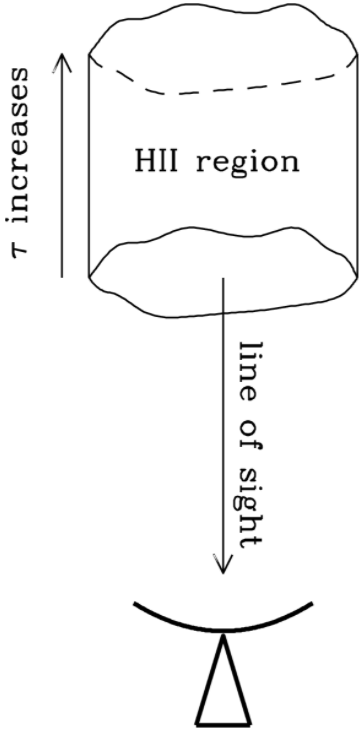
\includegraphics[width=.3\linewidth]{Chapter_2/Figures/NRAO_radio4n7.png}
    \caption[The schematic picture of \ih~region]{\label{fig:nrao_radio4n7}
        This figure shows the schematic picture of the \ih~region.
        Astronomers often approximate \ih~regions by the uniform cylinders.
        Cylindrical assumption lets us to calculate optical depth $\tau$ easily.
    }
\end{figure}

\begin{equation}\label{eq:essential_radio4n53}
\tau=-\int\msb{los} \kappa\,\rd s \propto \int \frac{n\msb{e} n\msb{i}}{\nu^{2.1} T^{3/2}} \rd s \sim \int \frac{n\msb{e}^2}{\nu^{2.1} T^{3/2}} \rd s
\end{equation}
where $s$ is the depth of \ih~region parallel to the line of sight.

At low frequencies enough that $\tau \gg 1$, the \ih~region becomes opaque, and the spectrum approaches the blackbody.
In this case, the brightness temperature approaches the electron temperature $\brp{T\sim10^4\,\mr{K}}$ and its flux density $S$ is in the Rayleigh-Jeans limit $\brp{S \propto \nu^2}$.
On the other hand, at frequency $\tau \ll 1$, the \ih~region is transparent and $S \propto \frac{2kT\nu^2}{c^2}\tau\brp{\nu} \propto \nu^{-0.1}$.

I show the spectrum of free-free radiation in the \ih~region in Figure~\ref{fig:nrao_radio4n8}.

\begin{figure}[htbp]
	\centering
	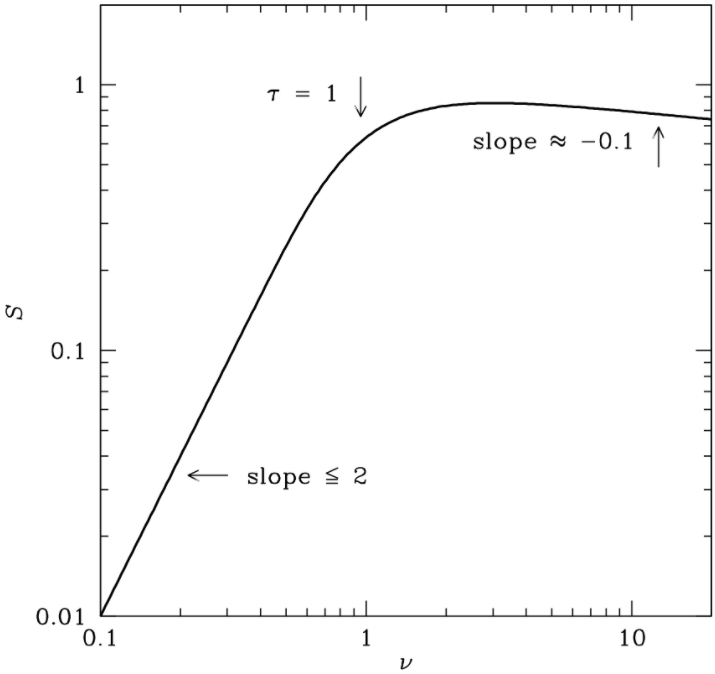
\includegraphics[width=.7\linewidth]{Chapter_2/Figures/NRAO_radio4n8.png}
    \caption[The spectrum of free-free radiation]{\label{fig:nrao_radio4n8}
        This figure shows the radio spectrum of free-free radiation.
        At low frequencies, we can see the blackbody with the slope $\leq 2$.
        The assumption of the uniform cylinder gives the slope $~2$, but the nonuniform \ih~region emits free-free radiation with the slope less than 2.
        At frequencies higher than the frequency of $\tau=1$, the slope is nearly flat $\brp{-0.1}$.
    }
\end{figure}

At low frequencies, the spectral index $\alpha$ on the log-log plot is useful to describe the density condition.
The definition of $\alpha$ is below:

\begin{equation}\label{eq:essential_radio4n55}
    \alpha \equiv \pm \frac{\rd \log S}{\rd \log \nu}
\end{equation}
where the sign depends on the literature.

With the $+$ sign convention, the spectral index of \ih~region well above the break frequency $\brp{\tau=1}$ is $\alpha=-0.1$.\\ \vspace{0.2cm}

Finally, I mention the idea of emission measure (EM) often used for understanding the physical condition in the \ih~region.
The definition of EM is

\begin{equation}\label{eq:essential_radio4n57}
    \frac{\mr{EM}}{\mr{pc} \cdot \mr{cm}^{-6}} \equiv \int\msb{los}\brp{\frac{n\msb{e}}{\mr{cm}^{-3}}}^2 \rd\brp{\frac{s}{\mr{pc}}}
\end{equation}

Then, we can write the optical depth $\tau$ in

\begin{equation}\label{eq:essential_radio4n58}
    \tau \sim 3.014 \times 10^{-2}\brp{\frac{T}{\mr{K}}}^{-3/2}\brp{\frac{\nu}{\mr{GHz}}}^{-2}\brp{\frac{\mr{EM}}{\mr{pc} \cdot \mr{cm}^{-6}}}\bra{g\msb{ff}}
\end{equation}
where $\bra{g\msb{ff}}$ is the free-free Gaunt factor:

\begin{equation}\label{eq:essential_radio4n59}
    \bra{g\msb{ff}} \sim \ln \brb{4.955 \times 10^{-2}\brp{\frac{\nu}{\mr{GHz}}}^{-1}}+1.5 \ln \brp{\frac{T}{\mr{K}}}
\end{equation}

\citet{Mezger1967} found the excellent approximation for the free-free opacity $\tau$ is

\begin{equation}\label{eq:essential_radio4n60}
    \tau \sim 3.28 \times 10^{-7}\brp{\frac{T}{10^4 \mr{K}}}^{-1.35}\brp{\frac{\nu}{\mr{GHz}}}^{-2.1}\brp{\frac{\mr{EM}}{\mr{pc} \cdot \mr{cm}^{-6}}}
\end{equation}

When we observe the break frequency $\nu$ $\brp{\tau \sim 1}$, then we can calculate EM with the electron temperature $\brp{\sim10^4\,\mr{K}}$.
And also, we can calculate the gas density in the \ih~region if we know its size (depth).





\section{Synchrotron radiation}\label{sec:synchrotronradiation}

Synchrotron radiation is a continuum emission which is usually dominant at less than $30\GHz$ in star-forming galaxies.
The interaction of high energy (relativistic) electrons accelerated by the supernova remnant or the galactic nuclei with the galactic magnetic field causes the radiation.
Since high energy electrons have a power-law energy distribution (not Maxwellian), we usually call the radiation ``non-thermal synchrotron radiation''.
If electrons have a much smaller velocity than the light, they emit the cyclotron radiation with the cyclotron frequency $\omega = \frac{eB}{m\msb{e}c}$ in cgs unit ($e$ is a charge, $B$ is the strength of the magnetic field, $m\msb{e}$ is a mass of an electron and $c$ is the speed of light).
In the normal star-forming galaxies ($B\sim10\mu G$), the electron gyro frequency is $30\,\mr{Hz}$ and we cannot observe it because it is much smaller frequency than the plasma frequency.

In this section, I show the mechanism to emit synchrotron radiation.
Firstly, I focus on synchrotron radiation emitted by a single electron.
Here, I use primed coordinates for the inertial frame in which an electron is at rest and unprimed coordinates for the frame of an observer at rest.
Then, I can write down the radiated power with Larmor's equation in the electron rest frame:

%Equation(5.24)
\begin{equation}\label{eq:essential_radio5n24}
    P^{\prime}=\frac{2\brp{e^{\prime}}^{2}\brp{a_{\perp}^{\prime}}^{2}}{3 c^{3}}=\frac{2 e^{2}\brp{a_{\perp}^{\prime}}^{2}}{3 c^{3}}
\end{equation}
where $e'=e$ because the electric charge is a relativistic invariant.

If an electron passes on $x$-axis in the magnetic field, its acceleration is only $y$ and $z$-axis because of the definition of Lorentz force.
Applying the chain rule to the acceleration by the magnetic field $a_{\perp} = \brp{a^2_y + a^2_z}^{1/2}$ in the rest frame of an observer yields

%Equation(5.25)
\begin{equation}\label{eq:essential_radio5n25}
    a_y \equiv \frac{\rd v_y}{\rd t}=\frac{\rd v_y}{\rd t^{\prime}} \frac{\rd t^{\prime}}{\rd t}=\frac{1}{\gamma} \frac{\rd v_y^{\prime}}{\rd t^{\prime}} \frac{\rd t^{\prime}}{\rd t}=\frac{a_y^{\prime}}{\gamma^2}\ \ \ \brp{a_z \equiv \frac{\rd v_z}{\rd t} = \frac{a'_z}{\gamma^2}}
\end{equation}

Then,

%Equation(5.26)
\begin{equation}\label{eq:essential_radio5n26}
    a_{\perp}=\frac{a_{\perp}^{\prime}}{\gamma^{2}}
\end{equation}

Thus,

%Equation(5.27)
\begin{equation}\label{eq:essential_radio5n27}
    P^{\prime}=\frac{2 e^{2}\brp{a_{\perp}^{\prime}}^{2}}{3 c^{3}}=\frac{2 e^{2} a_{\perp}^{2} \gamma^{4}}{3 c^{3}}
\end{equation}

Now, I need to transform $P' = \frac{\rd E'}{\rd t'}$ into $P = \frac{\rd E}{\rd t}$.
The chain rule derives

%Equation(5.28)
\begin{equation}\label{eq:essential_radio5n28}
    P \equiv \frac{\rd E}{\rd t}=\frac{\rd E}{\rd t^{\prime}} \frac{\rd t^{\prime}}{\rd t}=\frac{\rd E}{\rd E^{\prime}} \frac{\rd E^{\prime}}{\rd t^{\prime}} \frac{\rd t^{\prime}}{\rd t}=\gamma P^{\prime} \gamma^{-1}=P^{\prime}
\end{equation}
where the radiated power is also the relativistic invariant.

Consequently,

%Equation(5.29)
\begin{equation}\label{eq:essential_radio5n29}
    P=P^{\prime}=\frac{2 e^{2} a_{\perp}^{2} \gamma^{4}}{3 c^{3}} \quad\left(a_{\|}=0\right)
\end{equation}

To calculate $a_{\perp}$, $a_{\perp} = \frac{\rd v_{\perp}}{\rd t} = \omega_B v_{\perp}$.
Since electrons emitting synchrotron radiation are relativistic, the angular frequency $\omega_{B}$ is $\omega_B = \frac{eB}{\brp{\gamma m\msb{e}}c}$.
Then,

%Equation(5.31)
\begin{equation}\label{eq:essential_radio5n31}
    a_{\perp}=\frac{e B v_{\perp}}{\gamma m_{\mathrm{e}} c}=\frac{e B v \sin \alpha}{\gamma m_{\mathrm{e}} c}
\end{equation}
where $\alpha$ shows the pitch angle between the electron velocity and the magnetic field $B$.

Inserting Equation~\ref{eq:essential_radio5n31} into Equation~\ref{eq:essential_radio5n29} yields

%Equation(5.32)
\begin{equation}\label{eq:essential_radio5n32}
    P=\frac{2 e^{2}}{3 c^{3}} \gamma^{2} \frac{e^{2} B^{2}}{m_{\mathrm{e}}^{2} c^{2}} v^{2} \sin ^{2} \alpha
\end{equation}

For simplicity, this equation often is written in

%Equation(5.37)
\begin{equation}\label{eq:essential_radio5n37}
    P=2 \sigma_{\mathrm{T}} \beta^{2} \gamma^{2} c U_{B} \sin ^{2} \alpha
\end{equation}
where $\sigma\msb{T}$ is the Thomson cross-section of an electron, $\beta=\frac{v}{c}$ and $U_B$ is the magnetic energy density $\brp{U_B = \frac{B^2}{8\pi}}$.

Therefore, the synchrotron power radiated by a single electron depends on $\gamma$, $U_B$ and $\alpha$ ($\beta\sim1$ if $\gamma \gg 1$)

The relativistic electrons can have lifetimes of thousands to millions of years before losing their energy via synchrotron radiation or other physical processes.
During their lifetimes, electrons scatter with the galactic magnetic field and charged particles repeatedly.

In this case, the distribution of the pitch angle $\alpha$ becomes random and isotropic, and we can derive the averaged synchrotron power $\bra{P}$ per electron over all possible $\alpha$:

%Equation(5.38)
\begin{equation}\label{eq:essential_radio5n38}
    \bra{P} = 2 \sigma\msb{T} \beta^2 \gamma^2 c U_B\bra{\sin^2 \alpha} = \frac{4}{3}\sigma\msb{T} \beta^2 \gamma^2 c U_B
\end{equation}
where
%Equation(5.39-41)
\begin{equation}\label{eq:essential_radio5n39}
    \begin{aligned}
    \bra{\sin^2 \alpha} & \equiv \frac{\int \sin^2 \alpha \rd \Omega}{\int \rd \Omega}=\frac{1}{4\pi} \int \sin^2 \alpha \rd \Omega \\
                        &=\frac{1}{4\pi} \int {\phi=0}^{2\pi} \int_{\alpha=0}^{\pi} \sin^2 \alpha \sin \alpha \rd \alpha \rd \phi=\frac{1}{4\pi} 2 \pi \frac{4}{3} \\
                        &=\frac{2}{3}
    \end{aligned}
\end{equation}

Here I describe the beaming effect, which is the specific feature of synchrotron radiation due to the relativistic electrons.
The relation between $v_x$ at the frame of the observer (unprimed) and $v'_x$  at the rest frame of the electron (primed) is

%Equation(5.43-45)
\begin{equation}\label{eq:essential_radio5n43}
    \begin{aligned}
        v_x \equiv \frac{\rd x}{\rd t} &= \frac{\rd x}{\rd t^{\prime}} \frac{\rd t^{\prime}}{\rd t}=\gamma\brp{\frac{\rd x^{\prime}}{\rd t^{\prime}}+v \frac{\rd t^{\prime}}{\rd t^{\prime}}}\brp{\frac{\rd t}{\rd t^{\prime}}}^{-1} \\
                                       &=\gamma\brp{v_x^{\prime}+v}\brb{\gamma\brp{1+\frac{\beta}{c} \frac{\rd x^{\prime}}{\rd t^{\prime}}}}^{-1} \\
                                       &=\brp{v_x^{\prime}+v}\brp{1+\frac{\beta v_x^{\prime}}{c}}^{-1}
    \end{aligned}
\end{equation}

In the $y$-direction,

%Equation(5.46-47)
\begin{equation}\label{eq:essential_radio5n46}
    \begin{aligned}
        v_y \equiv \frac{\rd y}{\rd t} &= \frac{\rd y}{\rd t^{\prime}} \frac{\rd t^{\prime}}{\rd t}=\frac{\rd y^{\prime}}{\rd t^{\prime}}\brp{\frac{\rd t}{\rd t^{\prime}}}^{-1} \\
                                       &= \frac{v_y^{\prime}}{\gamma}\brp{1+\frac{\beta v_x^{\prime}}{c}}^{-1}
    \end{aligned}
\end{equation}

In the electron's rest frame, if an electron emits synchrotron photons with speed $c$ at an angle $\theta'$ from $x'$-axis, then the relation among $\theta'$, $v'$ and $c$ is

%Equation(5.48)
\begin{equation}\label{eq:essential_radio5n48}
    \cos \theta^{\prime}=\frac{v_x^{\prime}}{c}, \quad \sin \theta^{\prime}=\frac{v_y^{\prime}}{c}
\end{equation}

In the observer's rest frame, we can write in the same way:

%Equation(5.49)
\begin{equation}\label{eq:essential_radio5n49}
    \cos \theta=\frac{v_x}{c}, \quad \sin \theta=\frac{v_y}{c}
\end{equation}

Using Equation~\ref{eq:essential_radio5n43},~\ref{eq:essential_radio5n46},~\ref{eq:essential_radio5n48} and~\ref{eq:essential_radio5n49} to eliminate $v$ and $v'$ yields the relation between $\theta$ and $\theta'$:

%Equation(5.50 and 51)
\begin{equation}\label{eq:essential_radio5n50}
    \begin{aligned}
        \cos \theta &= \brp{\frac{v_x^{\prime}+v}{1+\beta v_x^{\prime} / c}} \frac{1}{c}=\brp{\frac{c \cos \theta^{\prime}+v}{1+\beta c \cos \theta^{\prime} / c}} \frac{1}{c}=\frac{\cos \theta^{\prime}+\beta}{1+\beta \cos \theta^{\prime}} \\
        \sin \theta &= \frac{v_y^{\prime}}{c \gamma\brp{1+\beta v_{x}^{\prime} / c}} = \frac{\sin \theta^{\prime}}{\gamma\brp{1+\beta \cos \theta^{\prime}}}
    \end{aligned}
\end{equation}

In the electron's rest frame, Larmor's equation implies a power pattern proportional to $\cos^2\theta'$ with nulls at $\theta'=\pm \frac{\pi}{2}$.

In the observer's rest frame, in this case:

%Equation(5.52)
\begin{equation}\label{eq:essential_radio5n52}
    \sin\theta = \frac{1}{\gamma} \quad \rightarrow \quad \theta=\pm \arcsin (1 / \gamma)
\end{equation}

Therefore, observers see synchrotron radiation from the electron in a narrow beam angle $\brp{\frac{2}{\gamma}}$ and this effect is called ``Beaming effect'' (Figure~\ref{fig:nrao_radio5n3})

%Figure(5.3)
\begin{figure}[htbp]
	\centering
	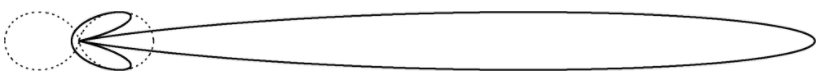
\includegraphics[width=.7\linewidth]{Chapter_2/Figures/NRAO_radio5n3.png}
    \caption[The schematic picture of relativistic aberration]{\label{fig:nrao_radio5n3}
        This figure shows the beaming effect which is a narrow angle for the radiation towards the observer.
        The dotted curve shows the original dipole power pattern of Larmor radiation and the solid line shows the case of $\gamma = 5$.
    }
\end{figure}

The beaming effect allows observers to see a short pulse of the radiation.
Note that the duration $\Delta t\msb{p}$ for observing the pulse is shorter than the time $\Delta t$, which the electron passes the narrow region $\brp{\frac{2}{\gamma}}$ because the electron moves toward the observer with the speed $\sim c$ (Figure~\ref{fig:nrao_radio5n4}).

%Figure(5.4)
\begin{figure}[htbp]
	\centering
	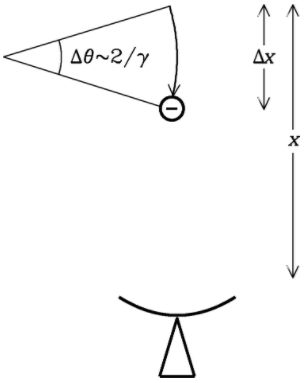
\includegraphics[width=.3\linewidth]{Chapter_2/Figures/NRAO_radio5n4.png}
    \caption[Simple condiguration of the synchrotron source and observer]{\label{fig:nrao_radio5n4}
        This figure shows the simple configuration of synchrotron radio source and the observer.
        During the time $\Delta t$ the electron moves $\Delta x = v\Delta t$ toward the observer, it almost keeps up with the radiation because it is relativistic.
    }
\end{figure}

%Equation(5.54, 55, 56)
\begin{equation}\label{eq:essential_radio5n54}
    \begin{aligned}
        \Delta t\msb{p} &=t(\text{end of observed pulse})-t(\text{start of observed pulse}) \\
                              &=\frac{\Delta x}{v}+\frac{(x-\Delta x)}{c}-\frac{x}{c} \\
                              &= \frac{\Delta x}{v}-\frac{\Delta x}{c}=\frac{\Delta x}{v}\left(1-\frac{v}{c}\right) \quad \ll \quad \frac{\Delta x}{v}=\Delta t
    \end{aligned}
\end{equation}

Replacing the total magnitude field by its perpendicular component $B_{\perp} = B\sin\alpha$ yields

%Equation(5.60)
\begin{equation}\label{eq:essential_radio5n60}
    \Delta t\msb{p} = \frac{1}{\gamma^2 \omega\msb{G} \sin \alpha}
\end{equation}
where $\alpha$ is the pitch angle of the electron.

Thus the synchrotron pulse is spiky with the halfwidth $\frac{\Delta t\msb{p}}{2} < 10^{-10}\,s$ and the time period is $\frac{\gamma}{\nu\msb{G} \brp{=\omega\msb{G} / 2\pi}} > 10^2\,s$ if $\gamma \sim 10^4$ and $B \sim 10\,\mr{\mu G}$ (Figure~\ref{fig:nrao_radio5n5}).

%Figure5.5
\begin{figure}[htbp]
	\centering
	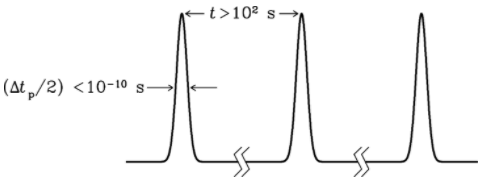
\includegraphics[width=.7\linewidth]{Chapter_2/Figures/NRAO_radio5n5.png}
    \caption[Synchrotron pulse by a single electron]{\label{fig:nrao_radio5n5}
        Synchrotron radiation by a single electron has a narrow pulses.
        Fourier transform of these pulses yields the power spectrum of synchrotron radiation (Equation~\ref{eq:essential_radio5n66}).
    }
\end{figure}


The synchrotron spectrum from a single electron is relatively flat at low frequencies and suddenly falls above

%Equation(5.65)
\begin{equation}\label{eq:essential_radio5n65}
    \nu_{\max} \sim \frac{1}{2 \Delta t\msb{p}} \sim \pi \gamma^2 \nu\msb{G} \sin \alpha \propto \gamma^2 B_{\perp}
\end{equation}

Once we know the pulse shape, we can derive the synchrotron power spectrum of a single electron by the Fourier transform as follows:

%Equation(5.66)
\begin{equation}\label{eq:essential_radio5n66}
    P\brp{\nu} = \frac{\sqrt{3} e^3 B \sin \alpha}{m\msb{e} c^2}\brp{\frac{\nu}{\nu\msb{c}}} \int_{\nu / \nu\msb{c}}^{\infty} K_{5/3}(\eta)\,\rd\eta
\end{equation}
 where $K_{5/3}$ is a modified Bessel function and $\nu_c$ is the critical frequency:

%Equation(5.67)
\begin{equation}\label{eq:essential_radio5n67}
    \nu\msb{c} = \frac{3}{2} \gamma^2 \nu\msb{G} \sin \alpha
\end{equation}

The spectrum shape of a single electron is shown in Figure~\ref{fig:nrao_radio5n6}.

%Figure(5.6)
\begin{figure}[htbp]
	\centering
	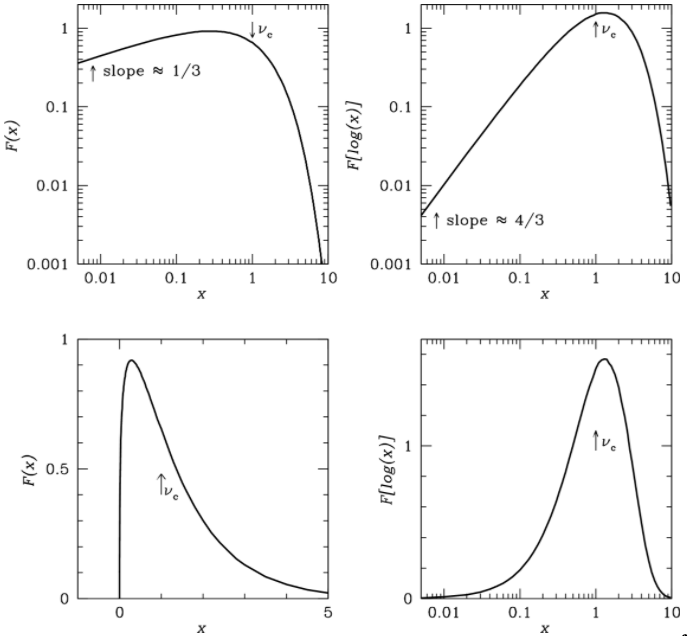
\includegraphics[width=.7\linewidth]{Chapter_2/Figures/NRAO_radio5n6.png}
    \caption[The synchrotron spectrum of a single electron]{\label{fig:nrao_radio5n6}
        These plots show the same function $F\brp{x} \equiv x\int^{\infty}_x K_{5/3}\brp{\eta}\,\rd\eta$ where $x \equiv \nu / \nu\msb{c}$ in different ways.
        In the log-log plot (upper left), we can see the spectral index is $1/3$ less than $x=1$ and it significantly falls above that.
    }
\end{figure}

Indeed, the property by a single electron smears out when we consider an ensemble of electrons due to a wide variety of their energies and pitch angles.


\subsection{Synchrotron Spectra of Optically Thin Radio Sources}\label{subsec:synchrotronspectra_opticallythin}
Here I consider the situation where a synchrotron source is optically thin ($\tau \ll 1$).
In this case, the spectrum of synchrotron radiation is a superposition of the spectra from individual distribution, and its flux density cannot rise faster than $\nu^{1/3}$ at any frequency $\nu$ (Figure~\ref{fig:nrao_radio5n6}).
We usually obtain the spectral index $\alpha\sim-0.75$ ($+$ sign convection) from the observation for most astrophysical sources of synchrotron radiation.
The energy distribution of high energy electrons is roughly a power-law from the theory of Fermi acceleration:

%Equation(5.70)
\begin{equation}\label{eq:essential_radio5n70}
    n(E) \rd E \propto E^{-\delta} \rd E
\end{equation}
where $n\brp{E}\rd E$ is the number of electrons whose energy is between $E$ and $E+\rd E$.

Here, I assume each electron emits the averaged power $\bra{P}$ (Equation~\ref{eq:essential_radio5n38}) with any energy $E$:

%Equation(5.71)
\begin{equation}\label{eq:essential_radio5n71}
    P=-\frac{\rd E}{\rd t}=\frac{4}{3} \sigma\msb{T} \beta^2 \gamma^2 c U_B
\end{equation}

at frequency $\nu \sim \gamma^2\nu\msb{G}$, which is close to the critical frequency $\nu\msb{c}$ (Equation~\ref{eq:essential_radio5n67}).
Then the emission coefficient of synchrotron radiation by an ensemble of electrons is

%Equation(5.73)
\begin{equation}\label{eq:essential_radio5n73}
    j_{\nu} \rd \nu=-\frac{\rd E}{\rd t} n(E) \rd E
\end{equation}
where $E = \gamma m\msb{e} c^2 \sim \brp{\frac{\nu}{\nu\msb{G}}}^{1/2} m\msb{e}c^2$.

Then we can write

%Equation(5.75)
\begin{equation}\label{eq:essential_radio5n75}
    \rd E \approx \frac{m\msb{e} c^2 \nu^{-1 / 2}}{2 \nu\msb{G}^{1 / 2}} \rd \nu
\end{equation}

so,

%Equation(5.76)
\begin{equation}\label{eq:essential_radio5n76}
    j_{\nu} \propto\brp{\frac{4}{3} \sigma\msb{T} \beta^2 \gamma^2 c U_B}\brp{E^{-\delta}}\brp{\frac{m\msb{e} c^2 \nu^{-1 / 2}}{2 \nu\msb{G}^{1 / 2}}}
\end{equation}

To investigate the frequency dependence of the emission coefficient $j_{\nu}$ on the frequency $\nu$ and the magnetic field $B$, I eliminate  $E$ and $\nu\msb{G}$ from the equation above, then

%Equation(5.77) and 5.78
\begin{equation}\label{eq:essential_radio5n77}
    \begin{aligned}
        j_{\nu} & \propto \brp{\frac{\nu}{\nu\msb{G}}} B^2 \brp{\frac{\nu}{\nu\msb{G}}}^{-\delta / 2} \brp{\nu \nu\msb{G}}^{-1 / 2} \propto \brp{\frac{\nu}{B}} B^2 \brp{\frac{\nu}{B}}^{-\delta / 2} \brp{\nu B}^{-1 / 2}\\
                & \propto B^{(\delta+1) / 2} \nu^{(1-\delta) / 2}
    \end{aligned}
\end{equation}

Consequently, the synchrotron radiation in the case of optically thin with the power-law distribution $\brp{n\brp{E} \propto E^{-\delta}}$ also has a power-law distribution and its spectral index $\alpha = \frac{1-\delta}{2}$.

In our galaxy, we observe $\alpha\sim-0.75$ around $1\GHz$ and then $\delta \sim 2.5$.



\subsection{Synchrotron Self-Absorption}\label{synchrotronselfabsorption}

The brightness temperature of synchrotron sources cannot exceed an absolute value at low frequencies, although most radio sources have the emission coefficient $j_{\nu} \propto \nu^{\alpha}$ (mostly in the case of optically thin: $\alpha\sim-0.75$ in $+$ sign convection).
If electrons in LTE and they have the Maxwellian energy distribution, they are thermal sources and their brightness temperatures equal to the electron's kinetic energy.

Here, I describe in the case where electrons are optically thick $\brp{\tau \gg 1}$.
In this case, synchrotron self-absorption happens and the spectral index changes into $\alpha = \frac{5}{2}$.

Firstly, I assume the critical frequency where most of the electrons with energy $E = \gamma m\msb{e} c^2$ emit the synchrotron radiation:

%Equation(5.80)
\begin{equation}\label{eq:essential_radio5n80}
    \nu_{\mathrm{c}} \sim \frac{\gamma^{2} e B}{2 \pi m_{\mathrm{e}} c}
\end{equation}

In the relativistic gas, the ratio between specific heats at constant pressure and volume is $\frac{c\msb{P}}{c\msb{V}}=\frac{4}{3}$ (nonrelativistic case: $\frac{5}{3}$).
So the relation between electron energy $E$ and electron temperature $T\msb{e}$ is

%Equation(5.82)
\begin{equation}\label{eq:essential_radio5n82}
    E=3 k T\msb{e}
\end{equation}

Thus, the effective temperature of relativistic electrons is defined below:

%Equation(5.83)
\begin{equation}\label{eq:essential_radio5n83}
    T\msb{e} \equiv \frac{E}{3 k}=\frac{\gamma m\msb{e} c^2}{3 k}
\end{equation}

Eliminating $\gamma$ from Equation~\ref{eq:essential_radio5n80} and~\ref{eq:essential_radio5n83} yields

%Equation(5.84)
\begin{equation}\label{eq:essential_radio5n84}
    T\msb{e} \approx \brp{\frac{2 \pi m\msb{e} c \nu}{e B}}^{1 / 2} \frac{m\msb{e} c^2}{3 k} \sim 1.18 \times 10^6\brp{\frac{\nu}{\mr{Hz}}}^{1/2}\brp{\frac{B}{\mr{gauss}}}^{-1/2}
\end{equation}

At sufficiently low frequency, the brightness temperature $T\msb{b}$ approaches the effective electron temperature $T\msb{e}$, and radio sources become opaque.
In the Rayleigh-Jeans limit, we can write $T\msb{b}$ as follows:

%Equation(5.87)
\begin{equation}\label{eq:essential_radio5n87}
    T\msb{b} \equiv \frac{I_{\nu}c^2}{2k\nu^2}
\end{equation}
where $I_{\nu}$ is the spectral brightness.

Substituting $T\msb{b} \sim T\msb{e}$ and Equation~\ref{eq:essential_radio5n84} yields:

%Equation(5.88)
\begin{equation}\label{eq:essential_radio5n88}
    I_{\nu} \sim \frac{2kT\msb{e}\nu^2}{c^2} \propto \nu^{1/2}\nu^2 B^{-1/2} = \nu^{5/2} B^{-1/2}
\end{equation}

Therefore, the self-absorbed synchrotron source has a spectral index $\alpha\sim\frac{5}{2}$ $\brp{S\brp{\nu} \sim \nu^{5/2}}$, which is independent of the slope $\delta$.

The spectrum of a homogeneous cylindrical synchrotron source is showed in Figure~\ref{fig:nrao_radio5n7}.

%Figure(5.7)
\begin{figure}[htbp]
	\centering
	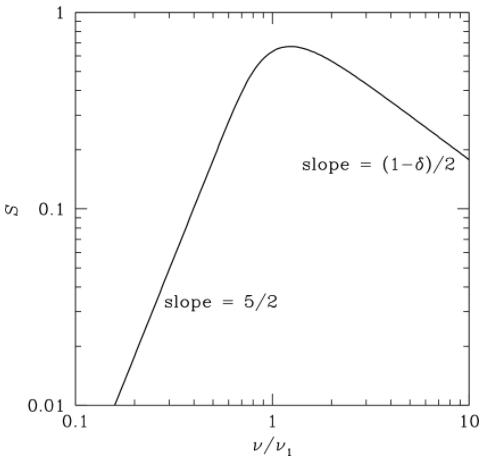
\includegraphics[width=.6\linewidth]{Chapter_2/Figures/NRAO_radio5n7.png}
    \caption[The spectrum of synchrotron radiation]{\label{fig:nrao_radio5n7}
        This figure shows the synchrotron spectrum.
        $\nu_1$ is the frequency at which $\tau=1$.
        The spectral index at the frequency $\nu$ above $\nu_1$ is $\brp{1-\delta}/2$.
        At lower frequencies less than $\nu_1$, we can see the synchrotron self-absorption with the slope $5/2$.
    }
\end{figure}

However, real radio sources have more complex shapes because they have nonuniform magnetic fields and electron energy distributions (Figure~\ref{fig:nrao_radio5n8}).

%Figure(5.8)
\begin{figure}[htbp]
	\centering
	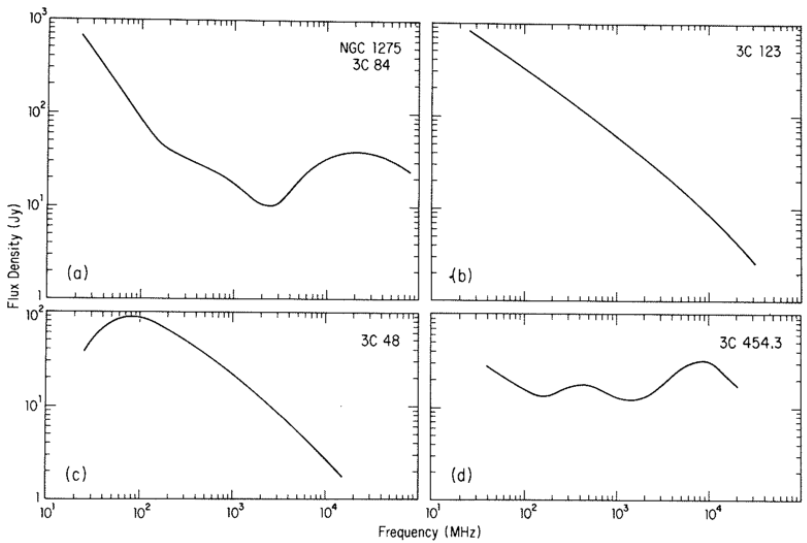
\includegraphics[width=.9\linewidth]{Chapter_2/Figures/NRAO_radio5n8.png}
    \caption[The spectrum of synchrotron radiation from real sources]{\label{fig:nrao_radio5n8}
        These plots show the radio spectra at low frequencies $\brp{10 \sim 10^5\MHz}$.
        Since real radio sources do not have uniform structures, these spectra look quite different from the uniform case (Figure~\ref{fig:nrao_radio5n7})
    }
\end{figure}
